% Figure 2 -- simplified VCF Core class diagram (the model VCF-RDFizer v3.1.0 emits).
% Classes and properties are taken from the ontology bundle vendored by v3.1.0
% (vocabulary commit 5bfd19d); only the backbone is drawn.
% Standalone TikZ source; build with: pdflatex vcf-core-classes.tex -> vcf-core-classes.pdf
% Drawn at the journal text width (372pt, about 13.1 cm) so it is included unscaled.
\documentclass[border=2pt]{standalone}
\usepackage[T1]{fontenc}
\usepackage{helvet}
\renewcommand{\familydefault}{\sfdefault}
\usepackage{tikz}
\usetikzlibrary{arrows.meta,positioning,calc,backgrounds}

\definecolor{chdr}{HTML}{FBE3E3}  \definecolor{chdrd}{HTML}{C00000}
\definecolor{crec}{HTML}{DDEFEF}  \definecolor{crecd}{HTML}{1F7F83}
\definecolor{csmp}{HTML}{DCE6F5}  \definecolor{csmpd}{HTML}{2F5597}
\definecolor{ccon}{HTML}{FCE4CC}  \definecolor{ccond}{HTML}{C55A11}
\definecolor{cfile}{HTML}{F6E3B4} \definecolor{cfiled}{HTML}{C9A227}
\definecolor{cband}{HTML}{F7F7F7}

\begin{document}
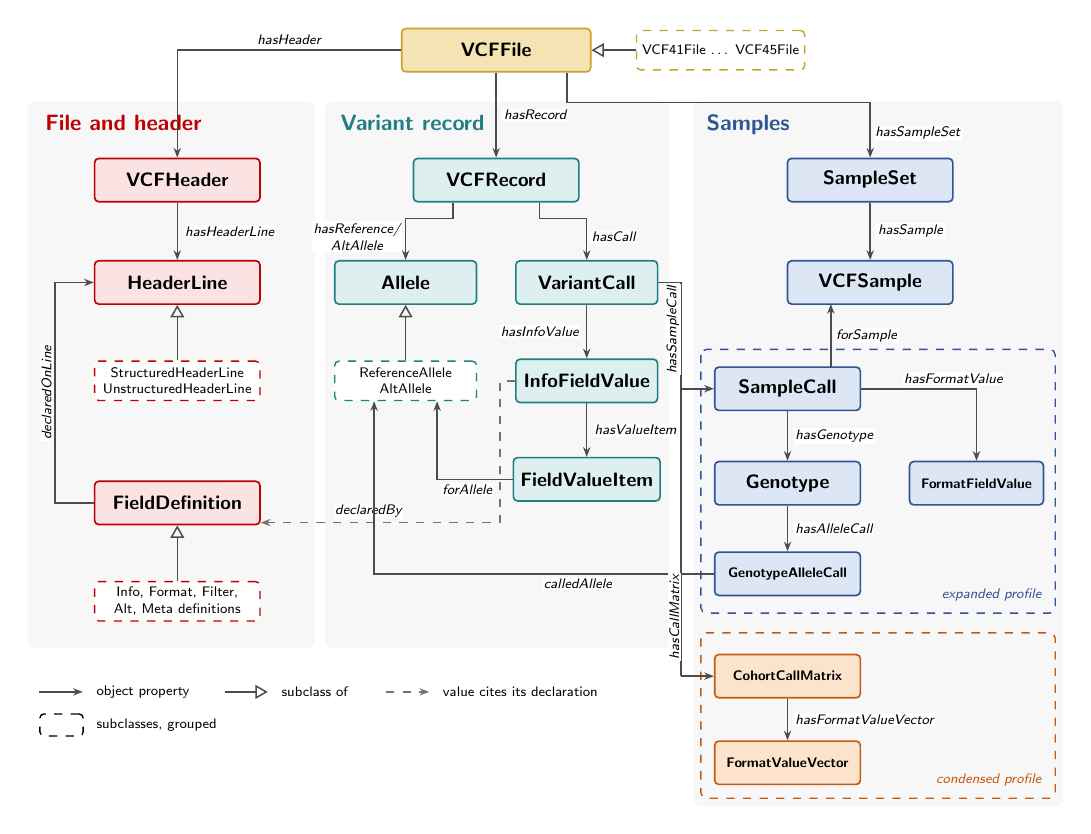
\begin{tikzpicture}[
  font=\scriptsize,
  cls/.style={draw, rounded corners=1.5pt, line width=0.6pt, align=center, inner sep=2.5pt,
              minimum height=0.55cm, minimum width=2.1cm, font=\scriptsize\bfseries},
  sub/.style={draw, dashed, rounded corners=1.5pt, line width=0.5pt, align=center, inner sep=2pt,
              minimum height=0.5cm, minimum width=2.1cm, font=\tiny},
  rel/.style={-{Stealth[length=3.5pt]}, line width=0.55pt, draw=black!70},
  isa/.style={-{Triangle[open, length=4.5pt, width=5pt]}, line width=0.55pt, draw=black!70},
  lnk/.style={-{Stealth[length=3.5pt]}, line width=0.5pt, draw=black!55, dashed},
  p/.style={font=\tiny\itshape, fill=white, inner sep=0.6pt},
  lane/.style={font=\footnotesize\bfseries\itshape, anchor=north west},
]

% ------------------------------------------------------------------ root
\node[cls, fill=cfile, draw=cfiled, minimum width=2.4cm] (file) at (5.9,-0.55) {VCFFile};
\node[sub, fill=white, draw=cfiled, minimum width=1.9cm] (filesub) at (8.75,-0.55) {VCF41File \dots\ VCF45File};
\draw[isa] (filesub) -- (file);

% ------------------------------------------------------------------ header layer
\node[lane, text=chdrd] at (0.05,-1.25) {File and header};
\node[cls, fill=chdr, draw=chdrd] (hdr) at (1.85,-2.2) {VCFHeader};
\node[cls, fill=chdr, draw=chdrd] (line) at (1.85,-3.5) {HeaderLine};
\node[sub, fill=white, draw=chdrd] (linesub) at (1.85,-4.75) {StructuredHeaderLine\\UnstructuredHeaderLine};
\node[cls, fill=chdr, draw=chdrd] (def) at (1.85,-6.3) {FieldDefinition};
\node[sub, fill=white, draw=chdrd] (defsub) at (1.85,-7.55) {Info, Format, Filter,\\Alt, Meta definitions};

\draw[rel] (file.west) -| node[p, pos=0.25, above=1pt]{hasHeader} (hdr.north);
\draw[rel] (hdr) -- node[p, right=2pt]{hasHeaderLine} (line);
\draw[isa] (linesub) -- (line);
\draw[isa] (defsub) -- (def);
\draw[rel] (def.west) -- (0.3,-6.3) -- node[p, sloped, above=0.5pt, pos=0.5]{declaredOnLine} (0.3,-3.5) -- (line.west);

% ------------------------------------------------------------------ record layer
\node[lane, text=crecd] at (3.8,-1.25) {Variant record};
\node[cls, fill=crec, draw=crecd] (rec) at (5.9,-2.2) {VCFRecord};
\node[cls, fill=crec, draw=crecd, minimum width=1.8cm] (allele) at (4.75,-3.5) {Allele};
\node[sub, fill=white, draw=crecd, minimum width=1.8cm] (allsub) at (4.75,-4.75) {ReferenceAllele\\AltAllele};
\node[cls, fill=crec, draw=crecd, minimum width=1.8cm] (call) at (7.05,-3.5) {VariantCall};
\node[cls, fill=crec, draw=crecd, minimum width=1.8cm] (info) at (7.05,-4.75) {InfoFieldValue};
\node[cls, fill=crec, draw=crecd, minimum width=1.8cm] (item) at (7.05,-6.0) {FieldValueItem};

\draw[rel] (file) -- node[p, right=2pt]{hasRecord} (rec);
\draw[rel] ($(rec.south)+(-0.55,0)$) |- ++(0,-0.2) -| node[p, pos=0.72, left=1pt, align=center]{hasReference/\\AltAllele} (allele.north);
\draw[rel] ($(rec.south)+(0.55,0)$) |- ++(0,-0.2) -| node[p, pos=0.72, right=1pt]{hasCall} (call.north);
\draw[isa] (allsub) -- (allele);
\draw[rel] (call) -- node[p, left=2pt]{hasInfoValue} (info);
\draw[rel] (info) -- node[p, right=2pt]{hasValueItem} (item);
\draw[rel] (item.west) -| node[p, pos=0.3, below=1pt]{forAllele} ($(allsub.south)+(0.4,0)$);
\draw[lnk] (info.west) -- (5.95,-4.75) -- (5.95,-6.55) -- node[p, pos=0.55, above=1pt]{declaredBy} (def.east |- 0,-6.55);

% ------------------------------------------------------------------ sample layer
\node[lane, text=csmpd] at (8.45,-1.25) {Samples};
\node[cls, fill=csmp, draw=csmpd] (set) at (10.65,-2.2) {SampleSet};
\node[cls, fill=csmp, draw=csmpd] (sample) at (10.65,-3.5) {VCFSample};
\draw[rel] ($(file.south)+(0.9,0)$) -- ++(0,-0.38) -| node[p, pos=0.78, right=1pt]{hasSampleSet} (set.north);
\draw[rel] (set) -- node[p, right=2pt]{hasSample} (sample);

% expanded profile
\node[cls, fill=csmp, draw=csmpd, minimum width=1.85cm] (scall) at (9.6,-4.85) {SampleCall};
\node[cls, fill=csmp, draw=csmpd, minimum width=1.7cm, font=\tiny\bfseries] (fval) at (12.0,-6.05) {FormatFieldValue};
\node[cls, fill=csmp, draw=csmpd, minimum width=1.85cm] (gt) at (9.6,-6.05) {Genotype};
\node[cls, fill=csmp, draw=csmpd, minimum width=1.85cm, font=\tiny\bfseries] (gac) at (9.6,-7.2) {GenotypeAlleleCall};
\draw[rel] (10.15,-4.575) -- node[p, right=1pt]{forSample} (10.15,-3.775);
\draw[rel] (scall.east) -| node[p, pos=0.4, above=1pt]{hasFormatValue} (fval.north);
\draw[rel] (scall) -- node[p, right=2pt]{hasGenotype} (gt);
\draw[rel] (gt) -- node[p, right=2pt]{hasAlleleCall} (gac);
\draw[rel] (gac.west) -| node[p, pos=0.2, below=1pt]{calledAllele} ($(allsub.south)+(-0.4,0)$);

% condensed profile
\node[cls, fill=ccon, draw=ccond, minimum width=1.85cm, font=\tiny\bfseries] (matrix) at (9.6,-8.5) {CohortCallMatrix};
\node[cls, fill=ccon, draw=ccond, minimum width=1.85cm, font=\tiny\bfseries] (vec) at (9.6,-9.6) {FormatValueVector};
\draw[rel] (matrix) -- node[p, right=2pt]{hasFormatValueVector} (vec);

% one trunk from the call into either profile
\draw[line width=0.55pt, draw=black!70] (call.east) -- (8.25,-3.5) -- (8.25,-8.5);
\draw[rel] (8.25,-4.85) -- (scall.west);
\draw[rel] (8.25,-8.5) -- (matrix.west);
\node[p, rotate=90, anchor=south] at (8.25,-4.1) {hasSampleCall};
\node[p, rotate=90, anchor=south] at (8.25,-7.75) {hasCallMatrix};

% lanes and profile frames
\begin{scope}[on background layer]
  \fill[cband, rounded corners=3pt] (-0.05,-1.2) rectangle (3.6,-8.15);
  \fill[cband, rounded corners=3pt] (3.72,-1.2) rectangle (8.1,-8.15);
  \fill[cband, rounded corners=3pt] (8.4,-1.2) rectangle (13.1,-10.15);
  \draw[csmpd, dashed, rounded corners=2pt, line width=0.5pt] (8.5,-4.35) rectangle (13.0,-7.7);
  \draw[ccond, dashed, rounded corners=2pt, line width=0.5pt] (8.5,-7.95) rectangle (13.0,-10.05);
\end{scope}
\node[font=\tiny\itshape, text=csmpd, anchor=south east] at (12.95,-7.67) {expanded profile};
\node[font=\tiny\itshape, text=ccond, anchor=south east] at (12.95,-10.02) {condensed profile};

% legend
\begin{scope}[shift={(0.1,-8.7)}]
  \draw[rel] (0,0) -- (0.55,0); \node[anchor=west, font=\tiny] at (0.6,0) {object property};
  \draw[isa] (2.35,0) -- (2.9,0); \node[anchor=west, font=\tiny] at (2.95,0) {subclass of};
  \draw[lnk] (4.4,0) -- (4.95,0); \node[anchor=west, font=\tiny] at (5.0,0) {value cites its declaration};
  \node[sub, minimum width=0.55cm, minimum height=0.28cm, inner sep=1pt] at (0.28,-0.42) {};
  \node[anchor=west, font=\tiny] at (0.6,-0.42) {subclasses, grouped};
\end{scope}
\end{tikzpicture}
\end{document}
